\documentclass[border=9pt]{standalone}
\usepackage[fontset=fandol]{ctex}
\usepackage{amsmath,amssymb,tikz}
\usetikzlibrary{arrows.meta,calc,decorations.pathmorphing}
\tikzset{arr/.style={-{Stealth[length=2mm]},semithick}}
\begin{document}

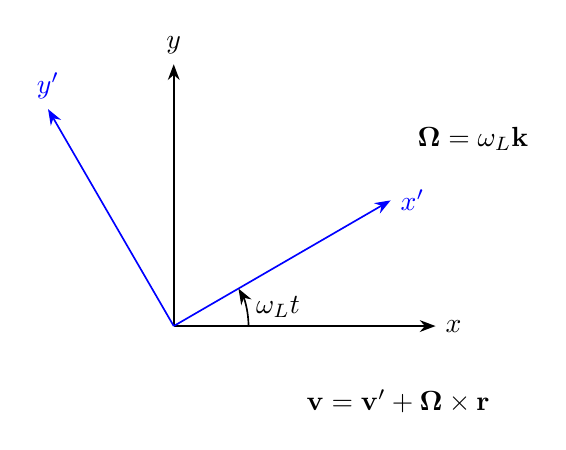
\begin{tikzpicture}[scale=.95]
\draw[arr](0,0)--(3.5,0)node[right]{$x$};\draw[arr](0,0)--(0,3.5)node[above]{$y$};
\draw[arr,blue](0,0)--(2.9,1.68)node[right]{$x'$};
\draw[arr,blue](0,0)--(-1.68,2.9)node[above]{$y'$};
\draw[arr](1,0)arc(0:30:1)node[midway,right]{$\omega_Lt$};
\node at(4,2.5){$\boldsymbol\Omega=\omega_L\mathbf k$};
\node at(3,-1){$\mathbf v=\mathbf v'+\boldsymbol\Omega\times\mathbf r$};
\end{tikzpicture}
\end{document}
